\chapter{Basics}
\label{chap:basics}
\section{ROS - The Robot Operating System}

The \textit{Robot Operating System} (ROS) is an open-source software framework providing a robust communication layer for distributed robot computing\cite{ros:intro}. Despite the name it is not an operating system in the traditional manner, as it does not provide or implement any processing, scheduling or data access functionality. It is a set of programs and libraries enabling developers to develop so-called \textit{nodes} that communicate with each other using the \textit{Publish-Subscribe-Pattern}.
This pattern allows multiple loosely-coupled nodes (applications) to exchange messages. This design allows a greater code-reuse since software for robots is written very modular\cite{Eugster2003}. For example, on a robot with a laser scanner and a motor, one node would decode the laser scanner data, publish the results to a specific topic which is subscribed by a controller node, that processes the data and then publishes motor control messages to another topic, which is again subscribed by the motor controller node. All nodes do not have to know each other. This makes it very easy to reuse the code for either the laser scanner or the motor driver node in other configurations (like multiple different robots) or exchange the controller node that processes the data. Using wireless connections, it is also possible to move specific processing tasks to external (\textit{Off-Board}) nodes. This comes in handy for example in terms of image processing, which is a task that usually overloads small on-board processing units built into robots.

The communication is organized by a program called \textit{ROS Core}. All nodes connect to this Core and tell it what they'd like to do (e.g. subscribing to topics, publishing to topics etc.). To reduce communication overhead, the actual data exchange is then done in a peer-to-peer manner, meaning the nodes directly exchange data with each other over TCP/IP. This also means that all nodes have to be able to reach each other, which might lead to problems when running ROS in bigger networks.

Sometimes, the publish-subscribe-pattern (and its inherent asynchrony) are not sufficient, as some calculations, which might be too heavy to be executed locally, might still have to be done synchronously. For this case, ROS introduces so-called \textit{services}. These are basically function calls that are offered by a node which may then be called by any other node over the network. These calls are executed synchronously and directly return a result.

Nodes have names seperated in so-called \textit{name spaces}. an example node name can look like in Listing \ref{code:ros:nodename}.
\begin{lstlisting}[caption={An example ROS node name},label=code:ros:nodename]
/robot/hand/controller
\end{lstlisting}


where \textit{/robot/hand} is the name space and \textit{controller} the node name. Topics and services do also have a specific name including a name space. This addressing scheme allows it to have multiple equally-called nodes or topics (e.g. for multiple sensors of the same type) by just putting them into different name spaces but preserving there names.

Numerous implementations of the ROS client libraries are available, the most common ones are developed and used in C/C++ and Python\cite{ros:client_libraries}. For developing a ROS-enabled Android application, an implementation of the ROS client library in Java is chosen. 

\subsection{rosjava / rosandroid}

There is an implementation of the ROS client library published on GitHub\footnote{\url{https://github.com/rosjava/rosjava_core}}. It includes support for all needed communication structures within ROS as well as the most common message types exchanged with ROS nodes. \textit{rosjava} is specifically designed to develop ROS-enabled Android applications and is originally developed by Google\cite{ros:rosjava:readme}.

The package \textit{rosandroid}\footnote{\url{https://github.com/rosjava/android_core}} is an extension of \textit{rosjava}. It offers functionalities to easily include ROS support into an Android application by offering readily usable \textit{Activities}\footnote{Activities are offering the user interface in Android applications} to connect the application to a ROS core or start an independent core within the application itself. It also includes some basic user controls like a joystick control which we will not make use of within this thesis.

\textit{rosandroid} is designed for the newest versions of Android, which leads to the fact that a small change has to be made in the code to make it compatible with older versions of Android, too. These changes are described in Chapter \ref{impl:compiling_rosandroid}.

\section{The Shadow C5 Robotic Hand}
% FOTO DER HAND
The \textit{Shadow C5 Robotic Hand} was developed by the \textit{Shadow Company}. It is designed to be as similar to a human hand as possible\cite{web:robothand:spec} in terms of force output, movement speed and movement sensitivity. It has 24 degrees-of-freedom, all controlled by 48 pneumatic muscles. These muscles, when pressurized, contract a little, applying force to the elements of the mechanical hand over imitated tendons. The developers tried to design the product as close to the average human forearm as they could. It weighs about 4kg and has a maximum movement speed of about half the speed at the joints a human could reach. The pneumatic muscles work with a pressure of 3.5 bar and having a maximum flow of 24 litres per minute, resulting in the need of a relatively powerful air compressor and air pipe system installed near the hand. Joint angles of all joints (controllable as well as non-controllable) are measured by hall-sensors at an accuracy of 0.2 degrees.
A similar robotic hand powered by electrical motors instead of pneumatic muscles is also present at the TAMS group at the University of Hamburg. This thesis will, however, mainly work with the pneumatic powered hand. 

\subsection{Integration into ROS}

\begin{wrapfigure}{L}{0.4\textwidth}
	\caption{\label{fig:hand:ros_integration}Schematic overview of the hand's integration into a ROS environment}
	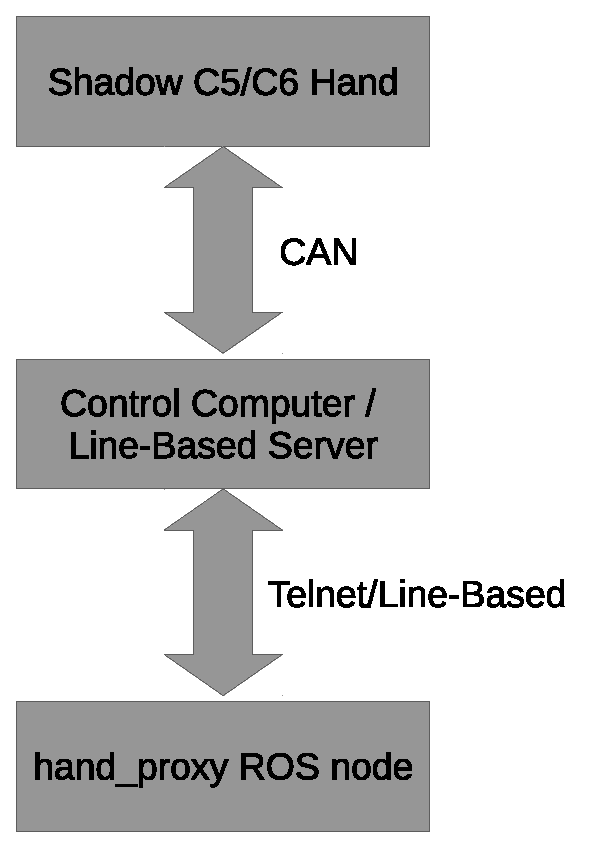
\includegraphics[width=0.4\textwidth]{assets/chpt_basics/hand/ros_integration.eps}
\end{wrapfigure}

The Shadow Robotic Hand possesses by default a CAN\footnote{Controller Area Network}-Bus interface over which it is controlled\cite{web:robothand:spec}. The CAN protocol has been implemented using a parallel port on a distinct machine next to the robotic hand. To have the ability to communicate with the hand over network, a server application has been implemented by members of the TAMS group at University of Hamburg. The line-based protocol implemented by this server is described in % TODO HIER REFERENZ EINFÜGEN
. Multiple applications have been developed to control the robotic hand without the integration of ROS. To make use of the features and advantages of a ROS environment, a ROS proxy was implemented. It basically listens to a ROS topic where it receives joint target states and publishes to another ROS topic where it sends the current measured joint angles to. The ROS hand proxy node communicates with the hand server over the line-based protocol and converts all data it receives for the corresponding other side. This set-up makes it easy to integrate the Shadow C6 hand into a ROS environment. See Figure \ref{fig:hand:ros_integration} for a schematic overview of how the robotic hand is integrated into ROS.

\begin{table}
	\caption{\label{tab:rosmsg:topics}Topics used to send and receive joint states}
	\begin{tabularx}{\linewidth}{|c|X|}
		\hline
		\textbf{/hand/joint\_states} & The ROS hand proxy publishes the current measured joint states it received from the hand server to this topic \\
		\hline
		\textbf{/hand/joint\_goals} & The ROS hand proxy receives packages containing joint states sent to this topic and passes it on to the hand server, causing the hand to try to reach the sent joint angles. \\
		\hline
	\end{tabularx}
\end{table}

The two important topics used throughout this thesis are denoted in Table \ref{tab:rosmsg:topics}. The message type used for both of these topics is \textit{sensor\_msgs/JointState}. These messages consist of the data fields denoted in Table \ref{tab:rosmsg:contents}. A few things are important to be considered while using the data contained in these messages. First, how the data is interpreted is application-specific. While the data fields contain arbitrary data it is important to know that the set-up used in this thesis only has rotating joints, meaning the data in the position field is in radians. For other types of joints (e.g. linear joints) this could possibly deviate. Second is, the order of elements is not important, however it is very important to maintain corresponding elements' positions at the same index within the \textit{names} and the \textit{position} fields. This means that e.g. the position for joint \textit{THJ1} must have the same index in the \textit{position} field as the string \textit{THJ1} in the \textit{names} field. Finally it is important to note that the \textit{effort} and \textit{velocity} fields are currently not used for the set-up. When these rules are followed it is easy to send joint states to the robot and observe its movement.

\begin{table}
	\caption{\label{tab:rosmsg:contents}Contents of the  \mbox{sensor\_msgs/JointState} message type}
	
	\begin{tabularx}{\linewidth}{|c|X|}
		\hline
		\textbf{Field} & \textbf{Description} \\
		\hline
		header & Header information including a time-stamp of when the message was sent and a sequence number of the message \\
		\hline
		names & Array of strings containing the joint names the other fields contain information about \\
		\hline
		position & Array of floats containing the position of each joint \\
		\hline
		velocity & Array of floats containing information about the velocity at which each joint is currently or shall be moving \\
		\hline
		effort & Array of floats containing information about with how much efford (e.g. force) a joint shall be or is moved \\
		\hline
	\end{tabularx}
\end{table}

\section{Inverse Kinematics}

Inverse kinematics is one of the challenging fields in many applications like robotics or computer animations\cite{Starke2017}. To understand what inverse kinematics is it is important to look at a robot (or e.g. animated figures in video games) from two different points of view. The normal viewer would describe the position and pose of a robot or effector in his own coordinate system, usually in Cartesian coordinates. This position can be described as an $n$-dimensional vector $X$. To describe movement of the robot, the viewer would then tell a difference between the new and the old position vectors $X_{new}-X=\Delta X$. A robot, however, often cannot move in Cartesian space, as it's kinematic chain (i.e. the parts of the robot connected by rotational or translational joints) can have $m$ degrees-of-freedom (DOF) with $m > n$. The position in the so-called \textit{joint-space} is referred to as $\theta$. To control such a robot with a high number of DOF, the controller has to be aware of the current position of the robot in Cartesian space $X$, the desired position change $\Delta X$ and the change in joint-space $\Delta \theta$ that has to be applied to the current position in joint space $\theta$. $\theta$ is known by the current state of the robot, finding $X$ is done by applying \textit{forward-kinematics} to $\theta$:
\begin{equation*}
	X = f(\theta)
\end{equation*}

Forward kinematics usually is a straight-forward process of beginning at the robot's base and iterating through all joints up to the \textit{end-effector} to find its position. The inverse kinematics to find the corresponding position in joint-space to reach the desired position in Cartesian space
\begin{equation*}
\theta = f^{-1}(X)
\end{equation*}
however is not as easy as the forward kinematics as with rising numbers of DOF no analytical solution is possible and multiple (up to an infinite number) valid joint-positions can exist - or even none at all\cite{DextquotesingleSouza}.

Many approaches to this problem have come up during the years. \citeauthor{andreasaristidou2009inverse} give a good overview over the existing methods in their technical report\cite{DextquotesingleSouza}.

\begin{figure}
	\caption{Forward and inverse kinematics\label{fig:basics:kinematics}}
	\begin{center}
		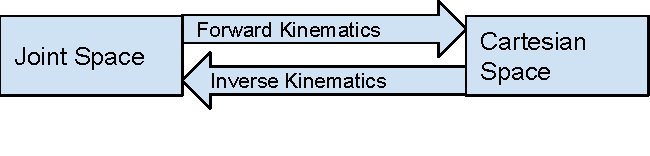
\includegraphics[width=0.6\textwidth]{assets/chpt_basics/Kinematics.pdf}
	\end{center}
\end{figure}

\subsection{BioIK}

BioIK is the name of a newly developed algorithm for inverse kinematics at the TAMS research group at the University of Hamburg\cite{Starke2017}. BioIK is a multi-goal evolutionary algorithm. This means in particular, that it accepts goals for multiple end-effectors in a kinematic chain whereas most other algorithms only accept one goal for one end-effector. This makes the algorithm especially suitable for highly articulated robots and models like humanoids\cite{Starkea2017}. Being an evolutionary algorithm means that solutions are created using predecessors and applying random mutation to a solution. Solutions of the algorithm are then classified by a fitness function, while good solutions remain within the so-called genom and bad solutions are not used for further evolutions\cite{Ruppel17} - similar to the so-called and name-giving real-world evolution. Within this thesis BioIK is used to calculate joint angles for given robot poses. The big advantage of BioIK is that it accepts multiple goals, i.e. one goal for every fingertip, and calculates corresponding joint positions based on the given goals.

\subsubsection{Integration into ROS}
Philipp Ruppel integrated BioIK into ROS during his Master Thesis. He integrated the BioIK solver into \textit{MoveIt!}, which is a motion planning framework integrated into ROS\cite{Coleman15}. Using \textit{MoveIt!} it is possible to plan motions and poses of robots from just calculating a pose of a robot to plan full motion trajectories from one pose to another while avoiding obstacles and collisions.

In addition to the functionality directly calling \textit{MoveIt!} interfaces from C++ a ROS service was implemented to get IK solutions from BioIK over a ROS service from arbitrary nodes - especially from non-C++ nodes like ones written in Java (rosjava, rosandroid) or Python (rospy)\footnote{The implementation of the ROS BioIK Service can be found at \url{https://gogs.crossmodal-learning.org/philipp.ruppel/bio_ik_service}}. 
Having this BioIK ROS service available makes it relatively easy to get IK solutions within nodes separated from \textit{MoveIt!} which is why it will be used within this thesis to request joint positions for given robot poses within the developed Android application. The process of integrating the service into the application is described in Chapter \ref{sec:robotarm:ctrl}.